\part{Aplicação das Técnicas de Elicitação de Requisitos}
\chapter[Aplicação das Técnicas de Elicitação de Requisitos]{Aplicação das Técnicas de Elicitação de Requisitos} \label{sec:tec}


Ainda com base nas mesmas ideias citadas no primeiro relatório sobre as síndromes endêmicas definidas por \cite{leffingwell2000managing}, as técnicas escolhidas baseadas nessas ideias foram, caso de uso, prototipagem e entrevista, as outras técnicas utilizadas foram escolhidas na mesma ideia mas com um adicional fator informal de experiência em trabalhos, por isso foram definidas somente ao início da segunda parte do projeto, são elas, análise e contexto, questionário, brainstorming e reunião informal.
Tanto o casos de uso quanto a prototipagem, foram usadas na validação com cliente ao final da fase de exploração. 

\section{Caso de uso}

Ao fim da fase de Exploração antes da análise de risco, foi feita uma validação junto ao cliente para confirmar sua visão sobre o sistema com o auxílio do diagrama de caso de uso. Esta técnica foi muito útil para maximizar a clareza da abstração do que era o sistema até aquele momento.

\section{Prototipagem}

Na fase de elicitação, para ajudar também na maximização da clareza acerca do sistema, foi usado a prototipagem de baixo nível para que o cliente já tivesse uma visão mais geral do site e pudesse opinar em nível de funcionalidades. Já num segundo momento, na fase de fundamentação, foi construído também um protótipo de alta fidelidade para que o cliente pudesse opinar em nível de layout e interface.

\subsection{Protótipo de baixa fidelidade}

O grupo de imagens \ref{fig:p1} é referente ao protótipo de baixa fidelidade do projeto.

\begin{figure}[!h]
	\centering
	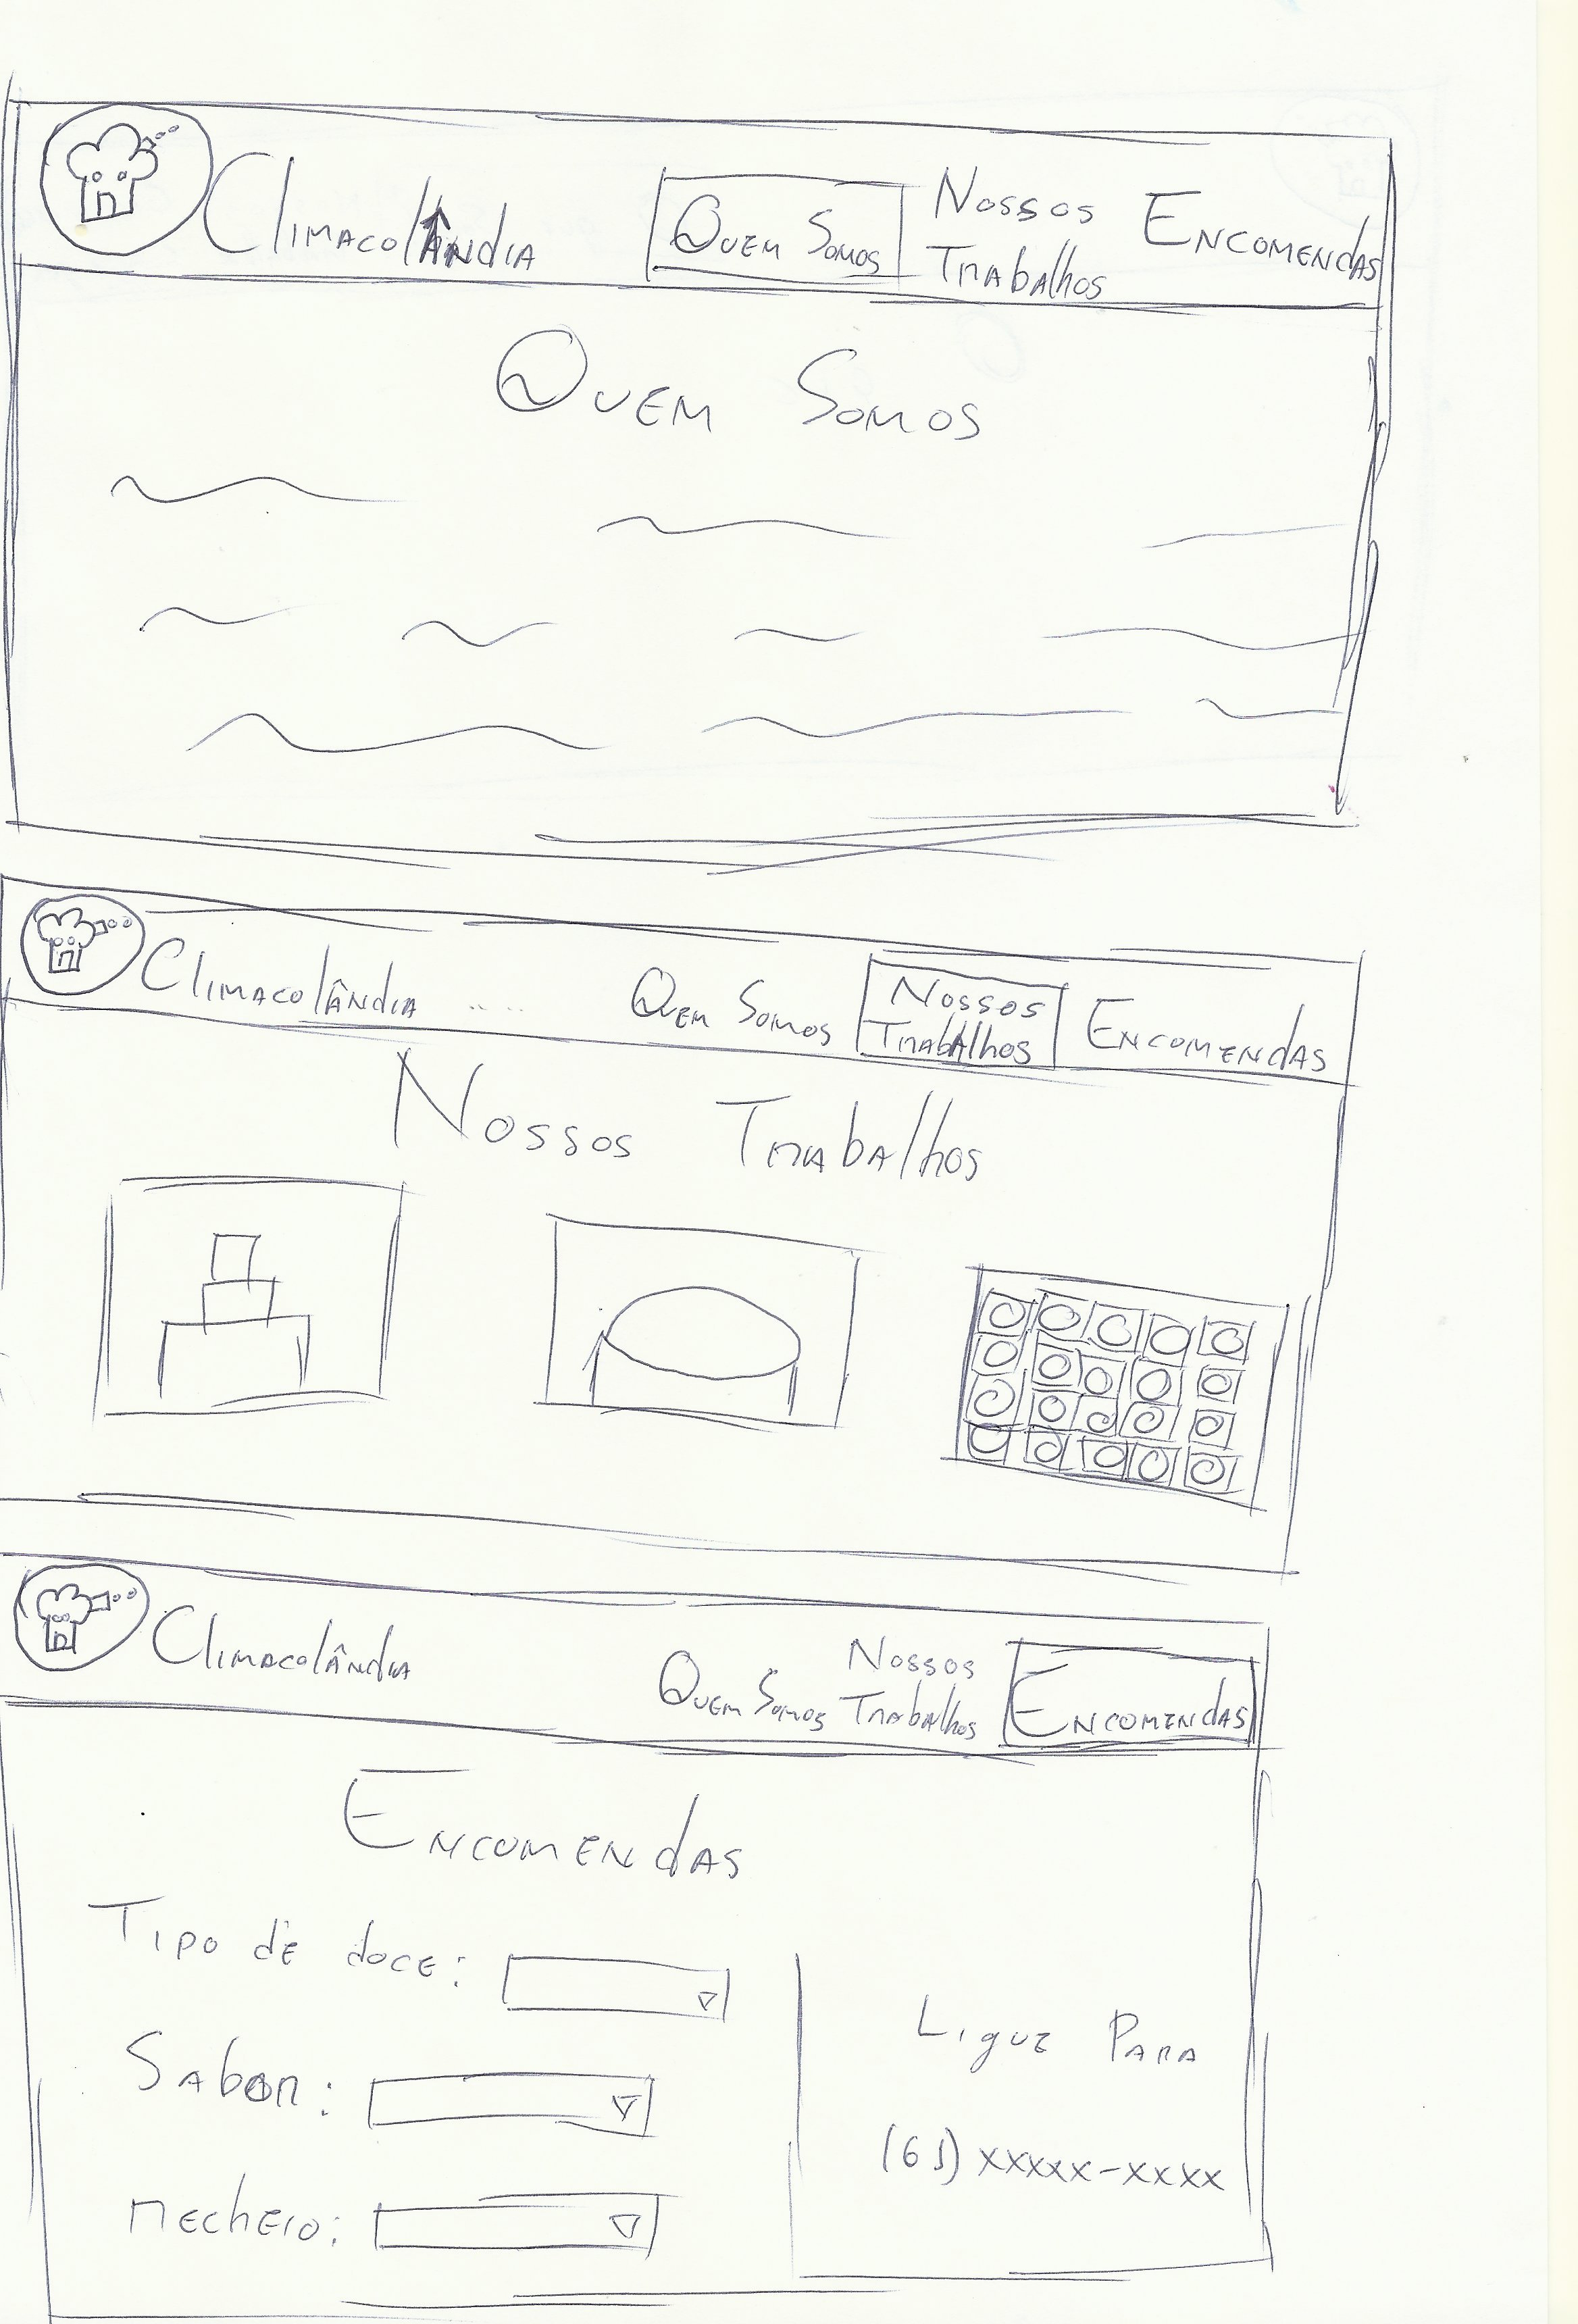
\includegraphics[width=.3\textwidth]{figuras/p1.png}
	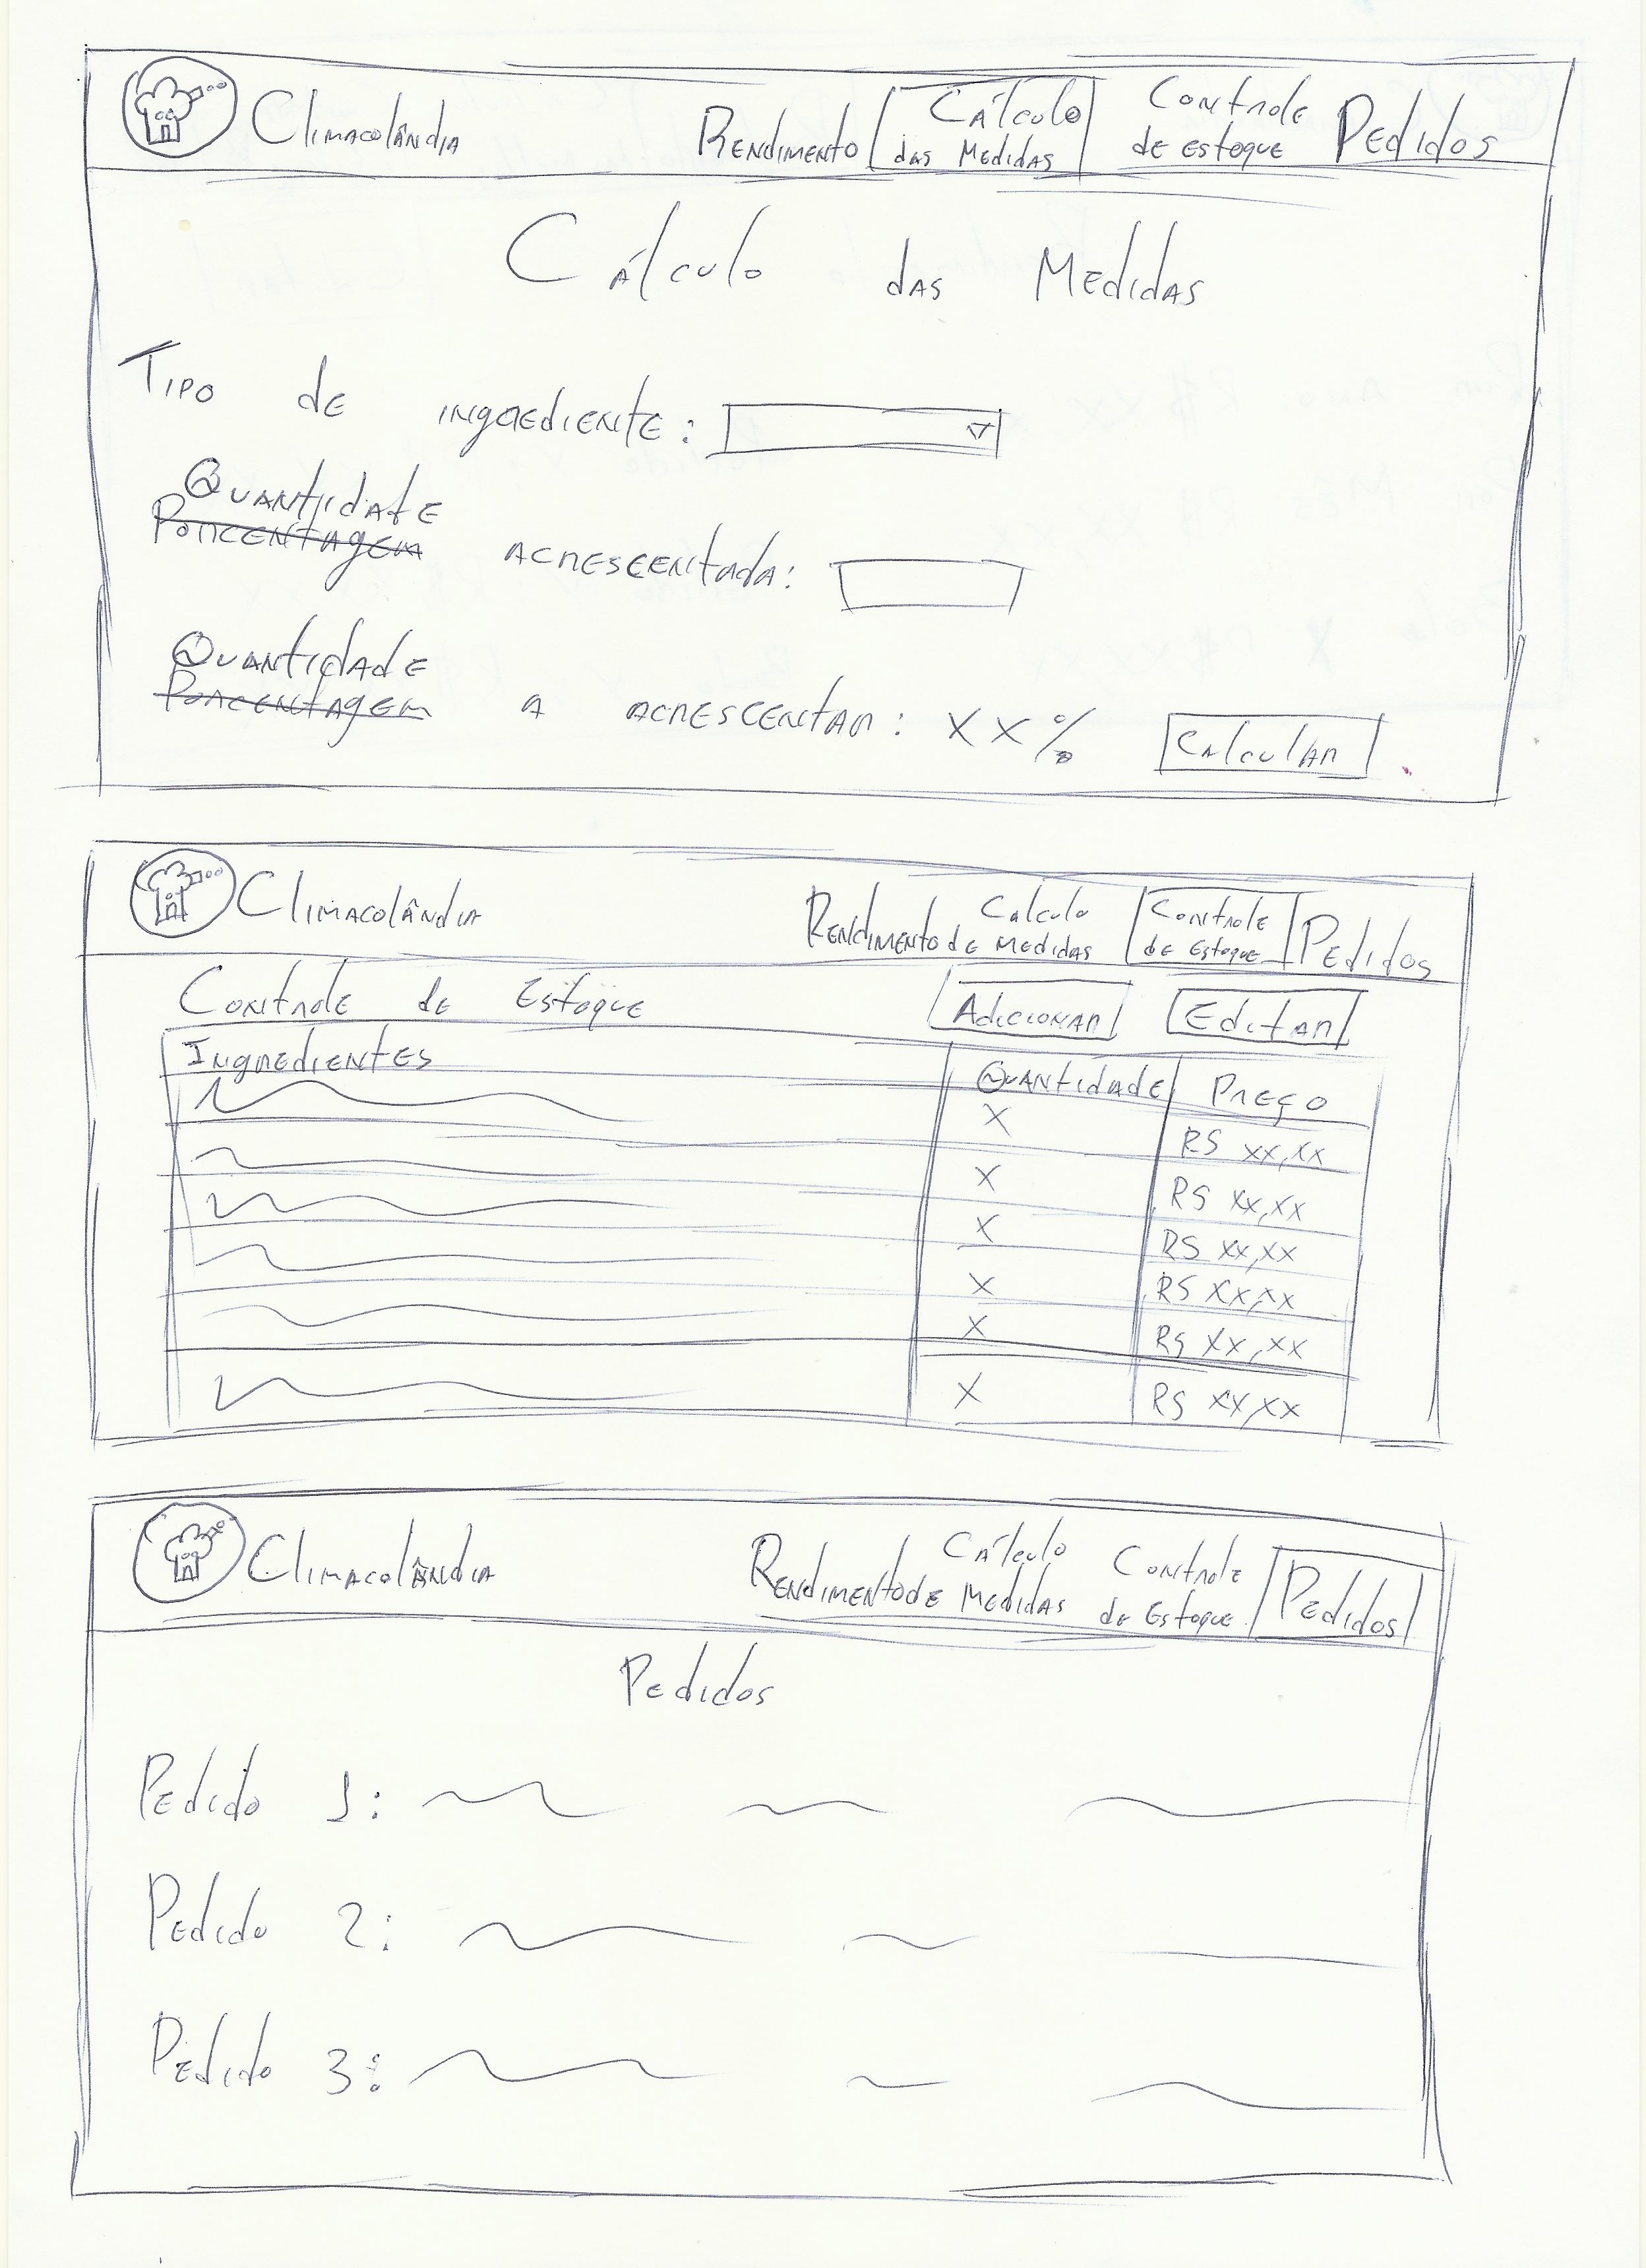
\includegraphics[width=.3\textwidth]{figuras/p2.JPG}
	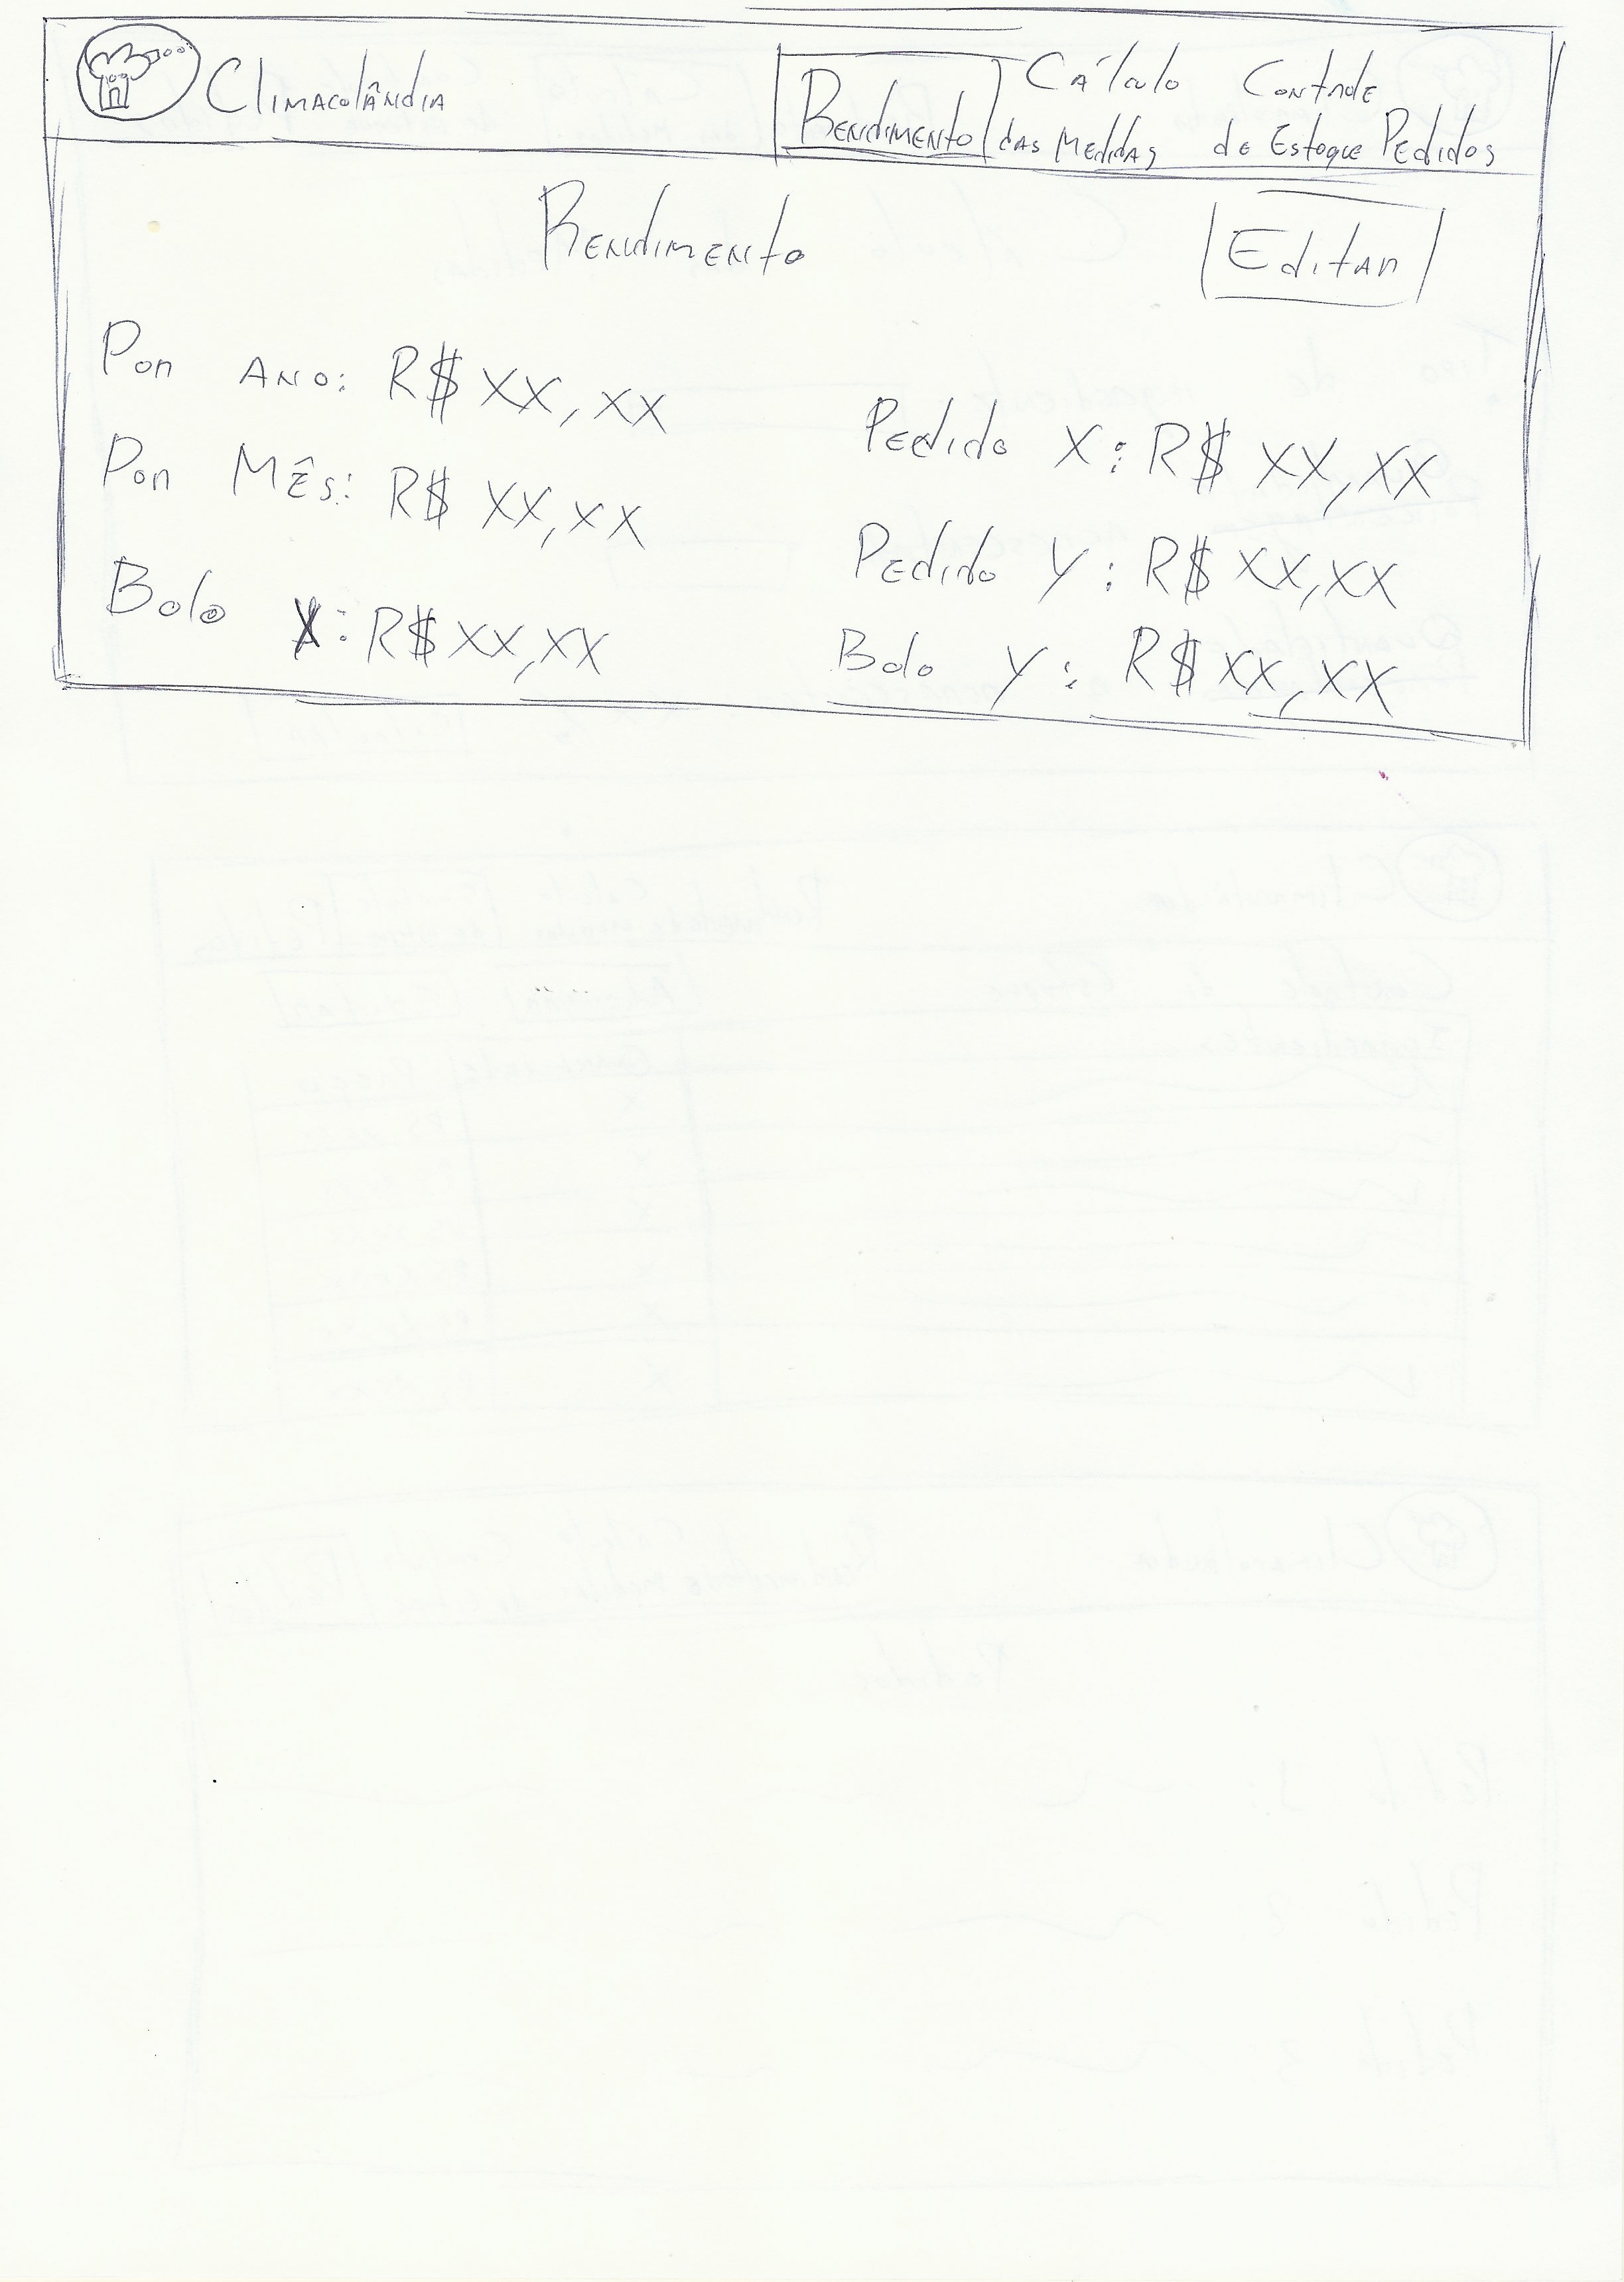
\includegraphics[width=.3\textwidth]{figuras/p3.JPG}
	\caption{Protótipo de baixa fidelidade}
	\label{fig:p1}
\end{figure}

\subsection{Protótipo de alta fidelidade}

O grupo de imagens \ref{fig:p2} é referente ao protótipo de alta fidelidade do projeto.

\begin{figure}[!h]
	\centering
	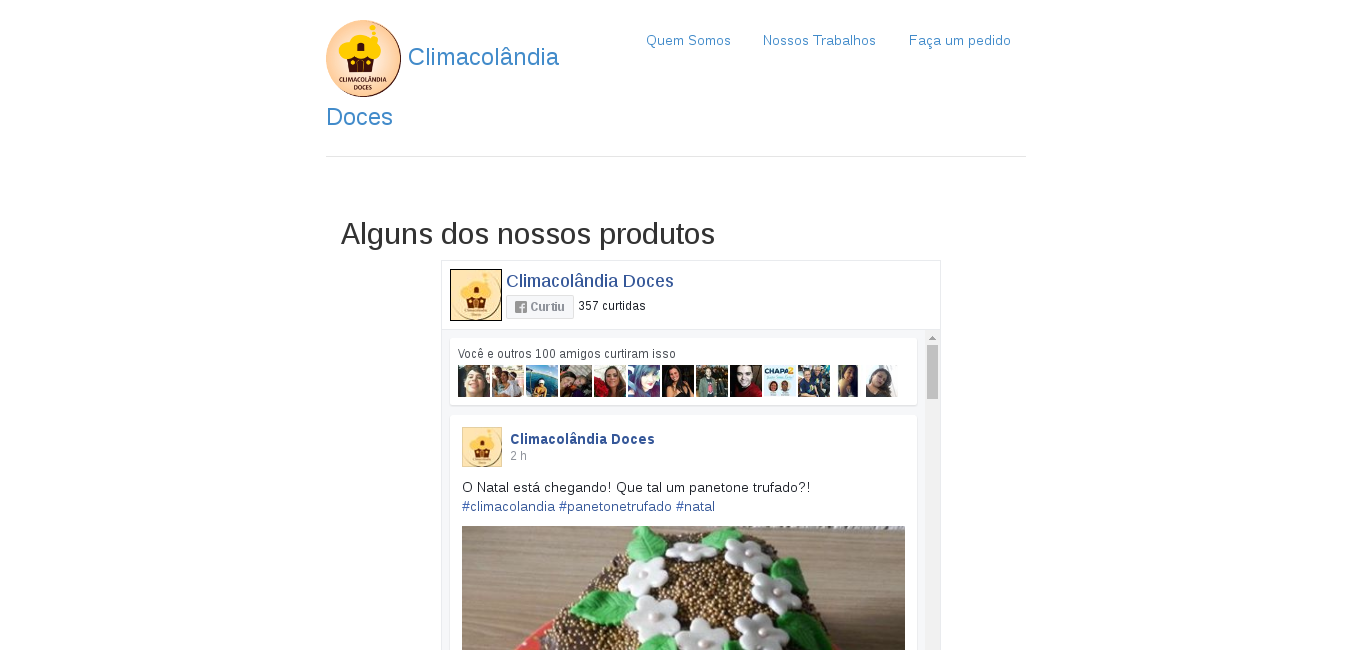
\includegraphics[width=.47\textwidth]{figuras/p4.png}
	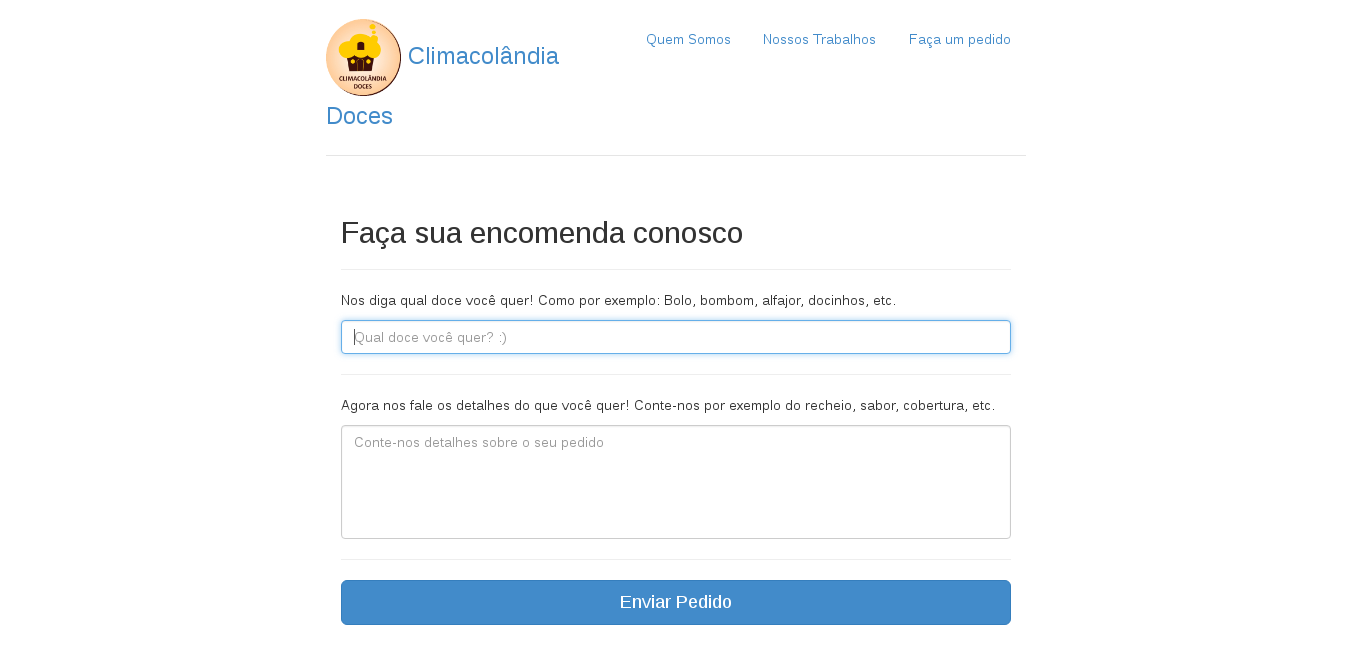
\includegraphics[width=.47\textwidth]{figuras/p5.png}
	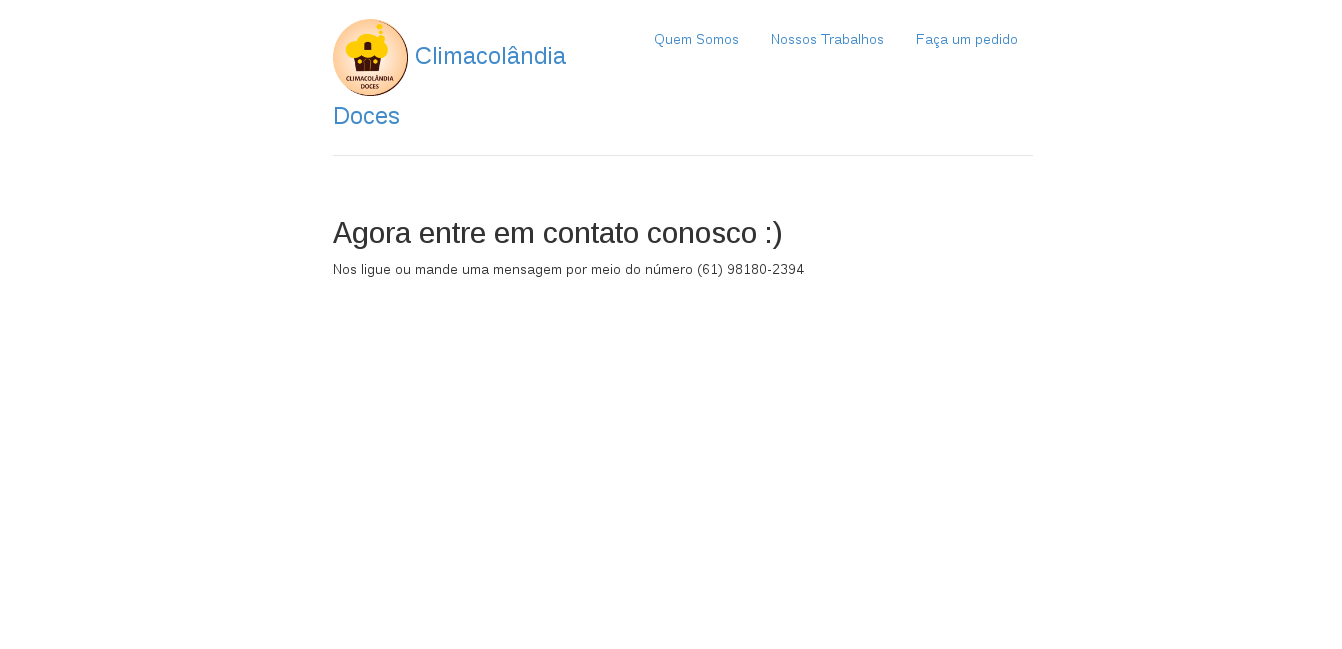
\includegraphics[width=.47\textwidth]{figuras/p6.png}
	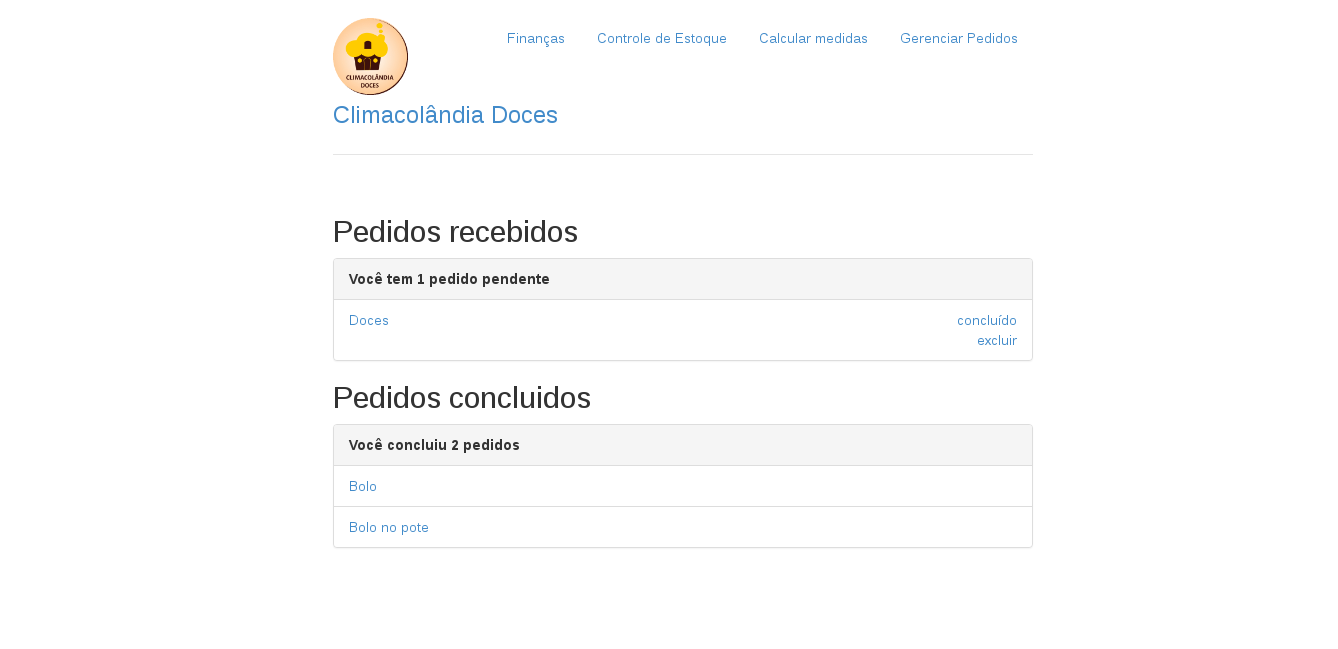
\includegraphics[width=.47\textwidth]{figuras/p7.png}
	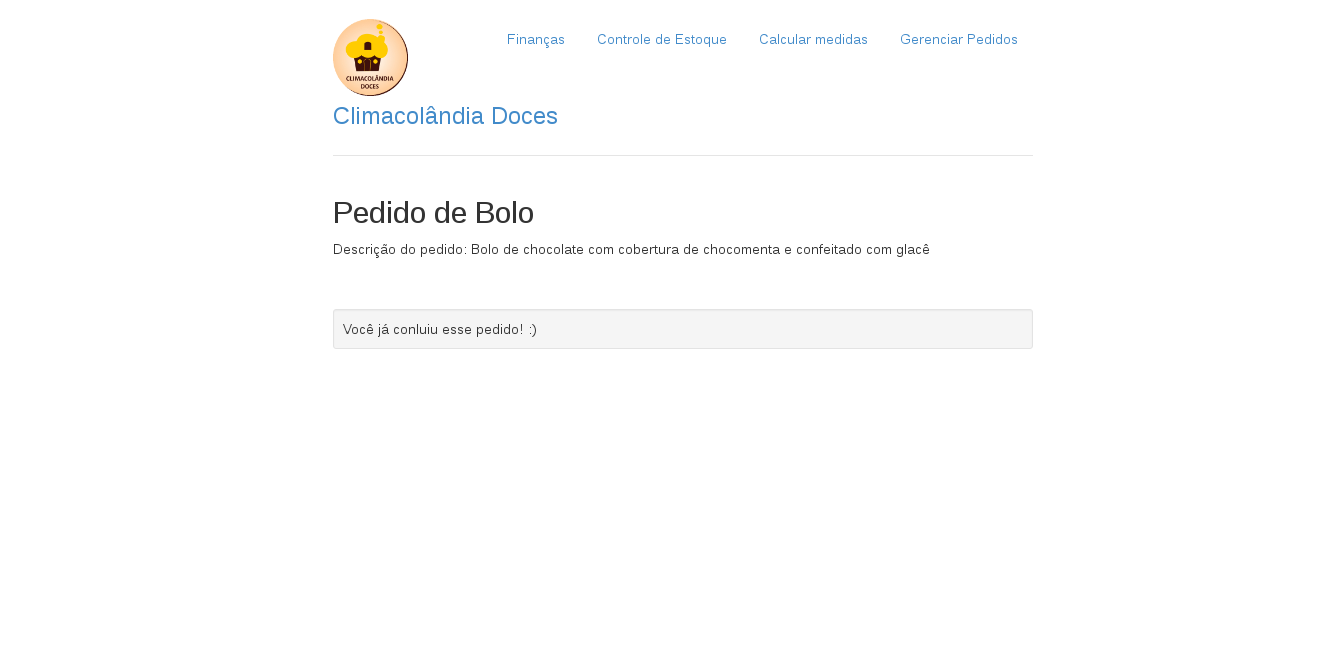
\includegraphics[width=.47\textwidth]{figuras/p8.png}
	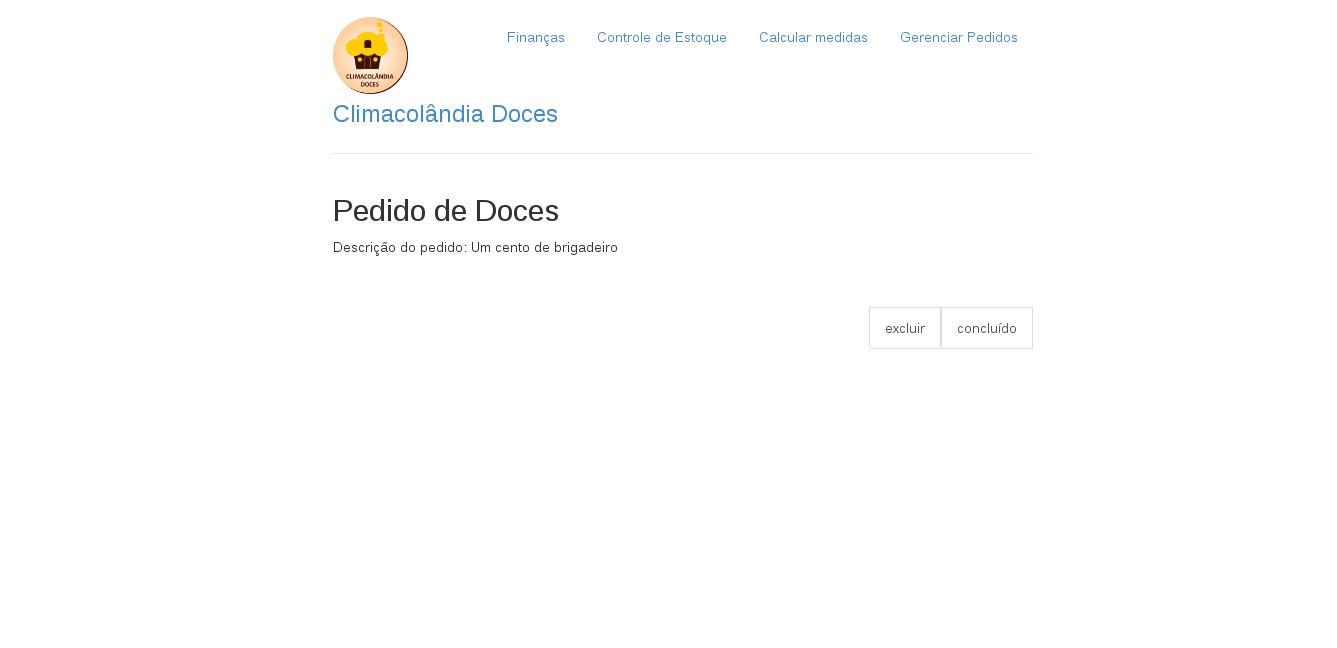
\includegraphics[width=.47\textwidth]{figuras/p9.png}
	\caption{Protótipo de Alta fidelidade}
	\label{fig:p2}
\end{figure}

\section{Entrevista}

Esta técnica foi usada por ser um método formal e mais organizado de coleta de informações,  por abranger da melhor forma, em visão do time, a compreensão de todo o contexto do projeto, por estar cara a cara com o cliente e assim poder analisar no mesmo momento as trocas de ideias de forma confortável e prática, como também, poder analisar as reações dos clientes com propostas de soluções e também pela facilidade em contato pessoal com o cliente a qualquer momento. Na única entrevista do projeto, a partir do início da segunda parte da disciplina, foram usadas a mais e juntamente para complementar toda a coleta de dados, a análise de contexto e o questionário.

A entrevista terá o objetivo principal em entender as reais necessidades dos mantenedores da empresa, anotando todos os problemas, soluções atuais e ideias de soluções futuras.

\subsection{Análise de Contexto}

Inicialmente, com o apoio da primeira reunião realizada na primeira fase do projeto, já compreendendo o ramo de negócios que seria inserido o projeto, é buscado o entendimento de como funciona o esquema completo de gestão da empresa para realizar uma comparação com as outras do mercado e assim entrar na fase de entrevistas na segunda parte do projeto com um conhecimento mais forte sobre o assunto para propor soluções mais completas e viáveis.

\subsection{Questionário}

Foi montado um questionário(tabela \ref{tab:quest}) com perguntas elaboradas por todos os integrantes do time de desenvolvimento sabendo desde o início da segunda fase do projeto que seria usado uma entrevista para o completo entendimento das necessidades dentro da fase de elicitação. As perguntas foram elaboradas no fato da empresa possuir apenas dois funcionários e ter tudo anotado em papel.

\begin{table}[!h]
\centering
\caption{Perguntas do questionário e suas respectivas respostas}
\label{tab:quest}
\resizebox{\textwidth}{!}{%
\begin{tabular}{|c|c|}
\hline
\rowcolor[HTML]{9B9B9B} 
Perguntas & Respostas \\ \hline
\begin{tabular}[c]{@{}c@{}}Na sua visão, quais são os maiores problemas \\ da empresa?\end{tabular} & \begin{tabular}[c]{@{}c@{}}A forma como é feito o controle da finanças \\ que é tudo em um caderninho então, muitas \\ vezes, não tenho nem o controle exato de \\ gastos e lucros. Um outro problema é que não \\ tenho o valor exato de quanto gasto em cada \\ confecção de doce e de certa forma todos os \\ dados da empresa são guardados em papel.\end{tabular} \\ \hline
\begin{tabular}[c]{@{}c@{}}Como gostaria que fosse resolvido o problema\\  de finanças?\end{tabular} & \begin{tabular}[c]{@{}c@{}}Um sistema que eu guardaria todo o gasto com \\ material e lucro com vendas e fizesse os \\ cálculos\end{tabular} \\ \hline
Como são realizados os pedidos? & Via mídias sociais ou pessoalmente \\ \hline
Como gostaria que fosse feito os pedidos? & \begin{tabular}[c]{@{}c@{}}De forma mais organizada mas que continue a \\ confirmação de forma direta\end{tabular} \\ \hline
Como são organizados os pedidos? & Anotando em papel com datas \\ \hline
\begin{tabular}[c]{@{}c@{}}Como gostaria que fosse feito a organização \\ dos pedidos?\end{tabular} & Um sistema que fizesse essa organização \\ \hline
Há um controle rigoroso de estoque? & \begin{tabular}[c]{@{}c@{}}Não, tudo é feito olhando, no momento da\\ produção, os armários que guardam os \\ materiais\end{tabular} \\ \hline
\begin{tabular}[c]{@{}c@{}}Gostaria que o sistema fizesse o controle desse \\ estoque e de quanto é gasto em cada produção?\end{tabular} & Sim \\ \hline
\begin{tabular}[c]{@{}c@{}}Gostaria de uma parte do sistema voltada para \\ o marketing de sua empresa?\end{tabular} & Sim, facilitaria muito mostrar meu trabalho \\ \hline
\end{tabular}%
}
\end{table}

\section{Reunião Informal}
\subsection{Primeira Reunião}

Foi realizada uma primeira reunião para compreensão do funcionamento geral da empresa, funcionários, marketing, todos os tipos de gestões etc, para assim podermos construir o primeiro relatório e ser possível trabalharmos em cima das necessidades e problemas propondo soluções ótimas aos nossos clientes, ou seja, esse foi o momento que abrangeu a análise de contexto dentro da primeira fase do trabalho. 

\subsection{Outras Reuniões}

Todas as demais reuniões foram realizadas apenas para as validações das atividades ao longo do projeto onde o cliente via rapidamente o que estava sendo feito e proposto e dava sua opinião, por sorte do grupo, o cliente aceitou todo o processo.

\subsubsection{Atas de reunião}
\subsubsubsection{Primeira reunião}

\begin{itemize}
\item Data: 25/08/2016	
\item Horário de Início: 19:30	
\item Horário de Término: 20:40
\item Presentes (Tabela \ref{tab:first1}):
\begin{table}[!h]
\centering
\caption{Pessoas presentes na primeira reunião}
\label{tab:first1}
\resizebox{\textwidth}{!}{%
\begin{tabular}{|c|c|c|}
\hline
\rowcolor[HTML]{9B9B9B} 
Nome & Área & Cargo \\ \hline
Elmar Roberto & Engenharia de Software & Gestão e Desenvolvimento \\ \hline
Gabriel Clímaco & Engenharia de Software & Gestão e Desenvolvimento \\ \hline
Gabriel Viana & Engenharia de Software & Gestão e Desenvolvimento \\ \hline
Matheus Henrique & Engenharia de Software & Gestão e Desenvolvimento \\ \hline
Cleide Marcia & Todo o processo de produção, marketing, gestão de finanças e estoque. & Dona, cozinheira, confeiteira, marketing, gestora. \\ \hline
\end{tabular}%
}
\end{table}
\item Local: casa dos donos da empresa
\item Discussão: Métodos de gestão da empresa, funcionários, tamanho da empresa, mercado de negócios, objetivos gerais da empresa e problemas. Todos esses tópicos se juntam na coleta da descrição do Contexto da Empresa
\begin{itemize}
\item Decisão: Sem tomada de decisão
\item Compromisso: Elaborar relatório 1 e realizar brainstorming para geração de ideias de soluções para os problemas se preparando para necessidades e assim futuramente refinar as ideias de soluções
\end{itemize}
\end{itemize}

\subsubsubsection{Segunda reunião}

\begin{itemize}
\item Data: 29/09/2016	
\item Horário de Início: 19:30	
\item Horário de Término: 21:00
\item Presentes (Tabela \ref{tab:first2}):
\begin{table}[!h]
\centering
\caption{Pessoas presentes na segunda reunião}
\label{tab:first2}
\resizebox{\textwidth}{!}{%
\begin{tabular}{|c|c|c|}
\hline
\rowcolor[HTML]{9B9B9B} 
Nome & Área & Cargo \\ \hline
Elmar Roberto & Engenharia de Software & Gestão e Desenvolvimento \\ \hline
Gabriel Clímaco & Engenharia de Software & Gestão e Desenvolvimento \\ \hline
Gabriel Viana & Engenharia de Software & Gestão e Desenvolvimento \\ \hline
Matheus Henrique & Engenharia de Software & Gestão e Desenvolvimento \\ \hline
Cleide Marcia & Todo o processo de produção, marketing, gestão de finanças e estoque. & Dona, cozinheira, confeiteira, marketing, gestora. \\ \hline
\end{tabular}%
}
\end{table}
\item Local: casa dos donos da empresa
\item Discussão: Necessidade
\begin{itemize}
\item Decisão: Organizar e separar necessidades
\item Compromisso: Levantar requisitos a partir das necessidades
\end{itemize}
\item Discussão: Solução
\begin{itemize}
\item Decisão: Construir um sistema web que abrange todos os problemas e detalhar todo o processo em documentos
\item Compromisso: Construir diagrama de casos de uso e descrevê-los junto com toda a documentação definida
\end{itemize}
\end{itemize}

\subsubsubsection{Terceira reunião}

\begin{itemize}
\item Data: 04/10/2016
\item Horário de Início: 19:30	
\item Horário de Término: 21:00
\item Presentes (Tabela \ref{tab:first3}):
\begin{table}[!h]
\centering
\caption{Pessoas presentes na terceira reunião}
\label{tab:first3}
\resizebox{\textwidth}{!}{%
\begin{tabular}{|c|c|c|}
\hline
\rowcolor[HTML]{9B9B9B} 
Nome & Área & Cargo \\ \hline
Elmar Roberto & Engenharia de Software & Gestão e Desenvolvimento \\ \hline
Gabriel Clímaco & Engenharia de Software & Gestão e Desenvolvimento \\ \hline
Gabriel Viana & Engenharia de Software & Gestão e Desenvolvimento \\ \hline
Matheus Henrique & Engenharia de Software & Gestão e Desenvolvimento \\ \hline
Cleide Marcia & Todo o processo de produção, marketing, gestão de finanças e estoque. & Dona, cozinheira, confeiteira, marketing, gestora. \\ \hline
\end{tabular}%
}
\end{table}
\item Local: casa dos donos da empresa
\item Discussão: Requisitos
\begin{itemize}
\item Decisão: Requisitos anotados adequadamente
\item Compromisso: Continuar com o projeto analisando os riscos e assim passando para a próxima fase
\end{itemize}
\end{itemize}

\subsubsubsection{Quarta reunião}

\begin{itemize}
\item Data: 13/10/2016	
\item Horário de Início: 19:30	
\item Horário de Término: 21:00
\item Presentes (Tabela \ref{tab:first4}):
\begin{table}[!h]
\centering
\caption{Pessoas presentes na quarta reunião}
\label{tab:first4}
\resizebox{\textwidth}{!}{%
\begin{tabular}{|c|c|c|}
\hline
\rowcolor[HTML]{9B9B9B} 
Nome & Área & Cargo \\ \hline
Elmar Roberto & Engenharia de Software & Gestão e Desenvolvimento \\ \hline
Gabriel Clímaco & Engenharia de Software & Gestão e Desenvolvimento \\ \hline
Gabriel Viana & Engenharia de Software & Gestão e Desenvolvimento \\ \hline
Matheus Henrique & Engenharia de Software & Gestão e Desenvolvimento \\ \hline
Cleide Marcia & Todo o processo de produção, marketing, gestão de finanças e estoque. & Dona, cozinheira, confeiteira, marketing, gestora. \\ \hline
\end{tabular}%
}
\end{table}
\item Local: casa dos donos da empresa
\item Discussão: Protótipo
\begin{itemize}
\item Decisão: Realizar um site com duas visões, uma para os donos da empresa e outra para seus clientes
\item Entregar um projeto com layout de sistema de loja para os donos e um layout de site padrão de vendas para seus clientes
\end{itemize}
\end{itemize}

\section{Análise dos dados coletados e propostas de solução}

Após cada reunião com o cliente foi e será realizado uma reunião apenas o grupo de trabalho na casa de algum dos integrantes, onde o local é definido logo após o término da reunião. Essa atividade tem a finalidade de analisar todos os dados coletados, organizando - os e propondo ideias de soluções para os problemas vistos dentro do contexto.
